% Por hacer:
% Mejorar las figuras en tikz

\begin{teo}
    Sea $f: [a,b] \rightarrow \R$ acotada y monótona\marginfootnote{Es decir, que sea creciente o decreciente en todo el intervalo $[a,b]$.}. Entonces $f \in \Rint$.
\end{teo}

\begin{proof}
    Sabemos por definición que
    
    \[
    L(f,P) = \sum_{j=1}^n m(f, I_j)|I_j|, \quad U(f,P) = \sum_{j=1}^n M(f, I_j)|I_j|
    \]
    
    \noindent ahora, como $f$ es monótona, nos permite razonar que $U(f,P) - L(f,P)$ es una suma telescópica.
    
    \begin{marginfigure}
        \centering
        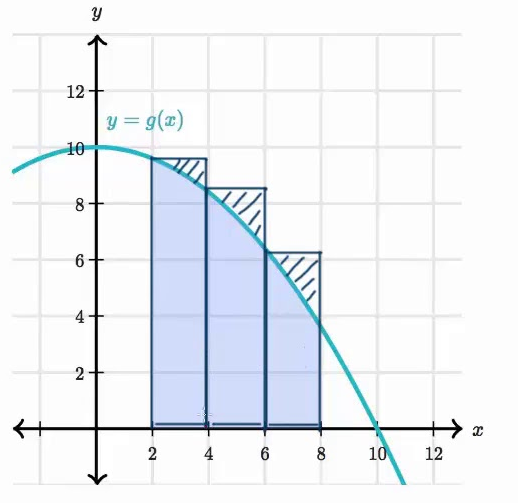
\includegraphics[scale=0.2]{img/cap3.png}
        \caption{\footnotesize Podemos ver aquí claramente, como por ejemplo para $I_1$ e $I_2$, $m(f, I_1) = M(f, I_2)$. Tomar en cuenta que para esta gráfica la función es decreciente, contrario a lo que se dice más adelante en el teorema.}
        
    \end{marginfigure}
    
    Luego, si $f$ es monótona creciente en todo el intervalo $[a,b]$
    
    \[
    U(f,P) - L(f,P) = M(f, I_n)|I_n| - m(f, I_1)|I_1|
    \]
    
    Ahora, para que $f$ sea integrable, necesitamos que $U(f,P) - L(f,P) = 0$ y para ello necesitamos que la diferencia $M(f, I_n)|I_n| - m(f, I_1)|I_1|$ sea arbitrariamente pequeña. En concreto, necesitamos
    
    \[
    M(f, I_n)|I_n| - m(f, I_1)|I_1| < \varepsilon
    \]
    
    \noindent para algún $\varepsilon > 0$. Para esto, consideremos una partición $P$ tal que
    
    \[
    |I_1| < \frac{\varepsilon}{2M}, \quad |I_n| < \frac{\varepsilon}{2M}
    \]
    
    \noindent donde $\displaystyle M = \sup_{x \in [a,b]} |f(x)|$. Así, tenemos
    
    \begin{align*}
        M(f, I_n)|I_n| &- m(f, I_1)|I_1| \leq M(f, I_n)\frac{\varepsilon}{2M} - m(f, I_1)\frac{\varepsilon}{2M} \\
        &< M\frac{\varepsilon}{2M} + M\frac{\varepsilon}{2M} = \varepsilon
    \end{align*}
    
    \noindent y así, tenemos que se cumple la desigualdad.
    
    Finalmente, haciendo tender $\varepsilon$ a cero, obtenemos que $U(f,P) = L(f,P)$ y en consecuencia $f$ es integrable.
\end{proof}

\begin{nota}
    Este número común $U(f, P) = L(f, P)$, recibirá el nombre de \ul{integral} de $f$ sobre $[a,b]$ y lo denotaremos por
    
    \[
    \intab f
    \]
\end{nota}

\begin{teo}[Condición de Riemann]\label{teo:condrie}
    Sea $f: [a,b] \rightarrow \R$ acotada en el intervalo $[a,b]$. Entonces $f$ es integrable sii dado $\varepsilon > 0$, $\exists \Pe$ tal que $U(f, \Pe) - L(f, \Pe) < \varepsilon$.
\end{teo}

\begin{proof}
    Para esta demostración, necesitaremos la propiedad de aproximación\marginfootnote{La propiedad de aproximación se enuncia de la siguiente manera:
    \begin{teo}
        Sea $A \subset \R$ acotada, entonces $\alpha = \sup A \iff \exists x_{\varepsilon} \in A: \alpha - \varepsilon \leq x_{\varepsilon} \leq \alpha$.
        
        Sea $A \subset \R$ acotada, entonces $\beta = \inf A \iff \exists x_{\varepsilon} \in A: \beta \leq x_{\varepsilon} < \beta + \varepsilon$.
    \end{teo}}.
    
    \begin{enumerate}
        \item ($\Rightarrow$) Como la función es integrable, entonces $\inf_P U(f,P) = \sup_P L(f, P)$. Gracias a la propiedad de aproximación para los supremos, sea $\varepsilon > 0$, escogemos una partición $P_0 \in \Pa([a,b])$ tal que
        
        \[
        \sup_P L(f,P) - \frac{\varepsilon}{2} < L(f,P_0) \leq \sup_P L(f,P)
        \]
        
        ahora, utilizando la hipótesis, la desigualdad queda como
        
        \begin{equation}\label{eq:condrie1}
            \inf_P U(f,P) - \frac{\varepsilon}{2} < L(f,P_0) \leq \inf_P U(f,P)
        \end{equation}
        
        Por otra parte, también tenemos que dado $\varepsilon > 0, \exists P_1:$
        
        \begin{equation}\label{eq:condrie2}
            \inf_P U(f,P) \leq U(f,P_1) \leq \inf_P U(f,P) + \frac{\varepsilon}{2}
        \end{equation}
        
        Definimos ahora $\Pe = P_0 \cup P_1$\marginfootnote{Lo que estamos diciendo acá es que $\Pe$ es refinamiento de $P_1$ y $P_0$.}, y cuando estimamos $U(f, \Pe) - L(f,\Pe)$, de \ref{eq:condrie1} y \ref{eq:condrie2} tenemos lo siguiente:
        
        \begin{align*}
            U(f,\Pe) &- L(f,\Pe) \leq U(f,P_1) - L(f,P_0) \\
            &\leq (\inf_p U(f,P) + \frac{\varepsilon}{2}) + (-\inf_P U(f,P) + \frac{\varepsilon}{2}) = \varepsilon
        \end{align*}
        
        \noindent en conclusión, $U(f,\Pe) - L(f,\Pe) < \varepsilon$.
        
        \item ($\Leftarrow$) Ahora nuestra hipótesis es: dado $\varepsilon > 0, \exists \Pe: U(f, \Pe) - L(f, \Pe) < \varepsilon$. Entonces, consideremos dicho $\varepsilon$ como $\varepsilon = 1/n (n \in \N)$, con el cual podemos tomar una partición $P_n$ canónica, con la cual podemos establecer lo siguiente:
        
        \[
        U(f, P_n) - L(f, P_n) < \frac{1}{n}
        \]
        
        Además, sabemos que
        
        \[
        \inf_P U(f,P) \leq U(f,P_n), \quad \sup_P L(f,P) \geq L(f,P_n)
        \]
        
        \noindent por la definición de supremo e ínfimo\marginfootnote{El ínfimo siempre será más pequeño que un elemento en particular del conjunto, y el supremo siempre será más grande que un elemento en particular del conjunto.}. De esta forma, tenemos que
        
        \[
        \inf_P U(f,P) - \sup_P L(f,P) \leq U(f, P_n) - L(f, P_n) < \frac{1}{n}
        \]
        
        \noindent en conclusión, tenemos que $\inf_P U(f,P) - \sup_P L(f,P) < \frac{1}{n}$, y si tomamos $n \to \infty$, entonces esa diferencia será tan pequeña como queramos. Más concretamente, por un lado tenemos que
        
        \[
        \inf_P U(f,P) - \sup_P L(f,P) < 0
        \]
        
        \noindent y por otro tenemos que
        
        \[
        \inf_P U(f,P) - \sup_P L(f,P) \geq 0
        \]
        
        \noindent en conclusión, no nos queda otra opción más que $\inf_P U(f,P) - \sup_P L(f,P) = 0$. Y esta es la definición de integrabilidad. Por lo que queda demostrado.
    \end{enumerate}
\end{proof}

\begin{cor}
    Sea $f: [a,b] \rightarrow \R$ acotada. $f$ es integrable si y solamente si:
    
    \[
    \lim_{n \to \infty} U(f, P_n) = \lim_{n \to \infty} L(f, P_n)\footnotemark
    \]\footnotetext{Esto es equivalente a $\int_a^b f$.}
\end{cor}

\begin{ejer}
    Demostrar el corolario anterior utilizando la condición de Riemann y la definición de límite.
\end{ejer}

\begin{teo}\label{teo:contint}
    Sea $f: [a,b] \rightarrow \R$ acotada. Si $f$ es continua, entonces $f \in \Rint$.
\end{teo}

\begin{proof}
    Como $[a,b]$ es un intervalo cerrado y acotado, y además estamos trabajando en los números reales, el intervalo es compacto, entonces la función $f$ además de ser continua, es \textbf{uniformemente continua}. Como la función es uniformemente continua en $[a,b]$, entonces dado $\varepsilon > 0, \exists \delta >0:$
    
    \[
    |f(x) - f(y)| < \frac{\varepsilon}{b-a} \quad \text{ si } \quad |x-y| < \delta \quad \footnotemark
    \]\footnotetext{Es importante elegir a $\varepsilon$ de esa manera. Esto es fundamental para la demostración.}
    
    \noindent y esto es cierto para todo par $x, y \in [a,b]$. Ahora sea $n \in \N$ tal que
    
    \[
    \frac{b-a}{n} < \delta
    \]
    
    \noindent si consideramos ahora que dado dicho $n \in \N$, a la partición canónica $P_n$ de $[a,b]$, entonces se cumplirá para todo $j=1, \dots, n$ lo siguiente
    
    \[
    |f(x) - f(y)| < \frac{\varepsilon}{(b-a)} \quad \text{para todos los $x$, $y$ de } I_j
    \]
    
    Bajo todas estas hipótesis, estimemos cuánto vale $U(f,P_n) - L(f,P_n)$. Sabemos que por definición esto es
    
    \[
    U(f,P_n) - L(f,P_n) = \sum_{j=1}^n \big( M(f,I_j) - m(f,I_j) \big)|I_j|
    \]
    
    \noindent escribiendo esto de otra manera, podemos decir que
    
    \begin{equation}\label{eq:cont1}
    U(f,P_n) - L(f,P_n) = \sum_{j=1}^n \big( f(z_j) - f(y_j) \big) \frac{(b-a)}{n}
    \end{equation}
    
    \noindent donde $z_j, y_j$ son tales que
    
    \[
    f(z_j) = M(f,I_j), \quad f(y_j) = m(f, I_j)
    \]
    
    Ahora, por la hipótesis de continuidad uniforme, y por nuestra elección del $\varepsilon$, podemos acotar la ecuación \ref{eq:cont1} de la siguiente manera
    
    \[
    U(f,P_n) - L(f,P_n) = \sum_{j=1}^n \big( f(z_j) - f(y_j) \big) \frac{(b-a)}{n} \leq \frac{1}{n} (b-a) \frac{\varepsilon}{b-a} < \varepsilon
    \]
    
    Finalmente, $U(f,P_n) - L(f,P_n) < \varepsilon$, lo que quiere decir que se cumple la condición de Riemann y $f$ es integrable.
\end{proof}